\section{Architectural design}

\subsection{Overview}
	\subsubsection{Context viewpoint}
	
		\begin{figure}[h]
			\centering
			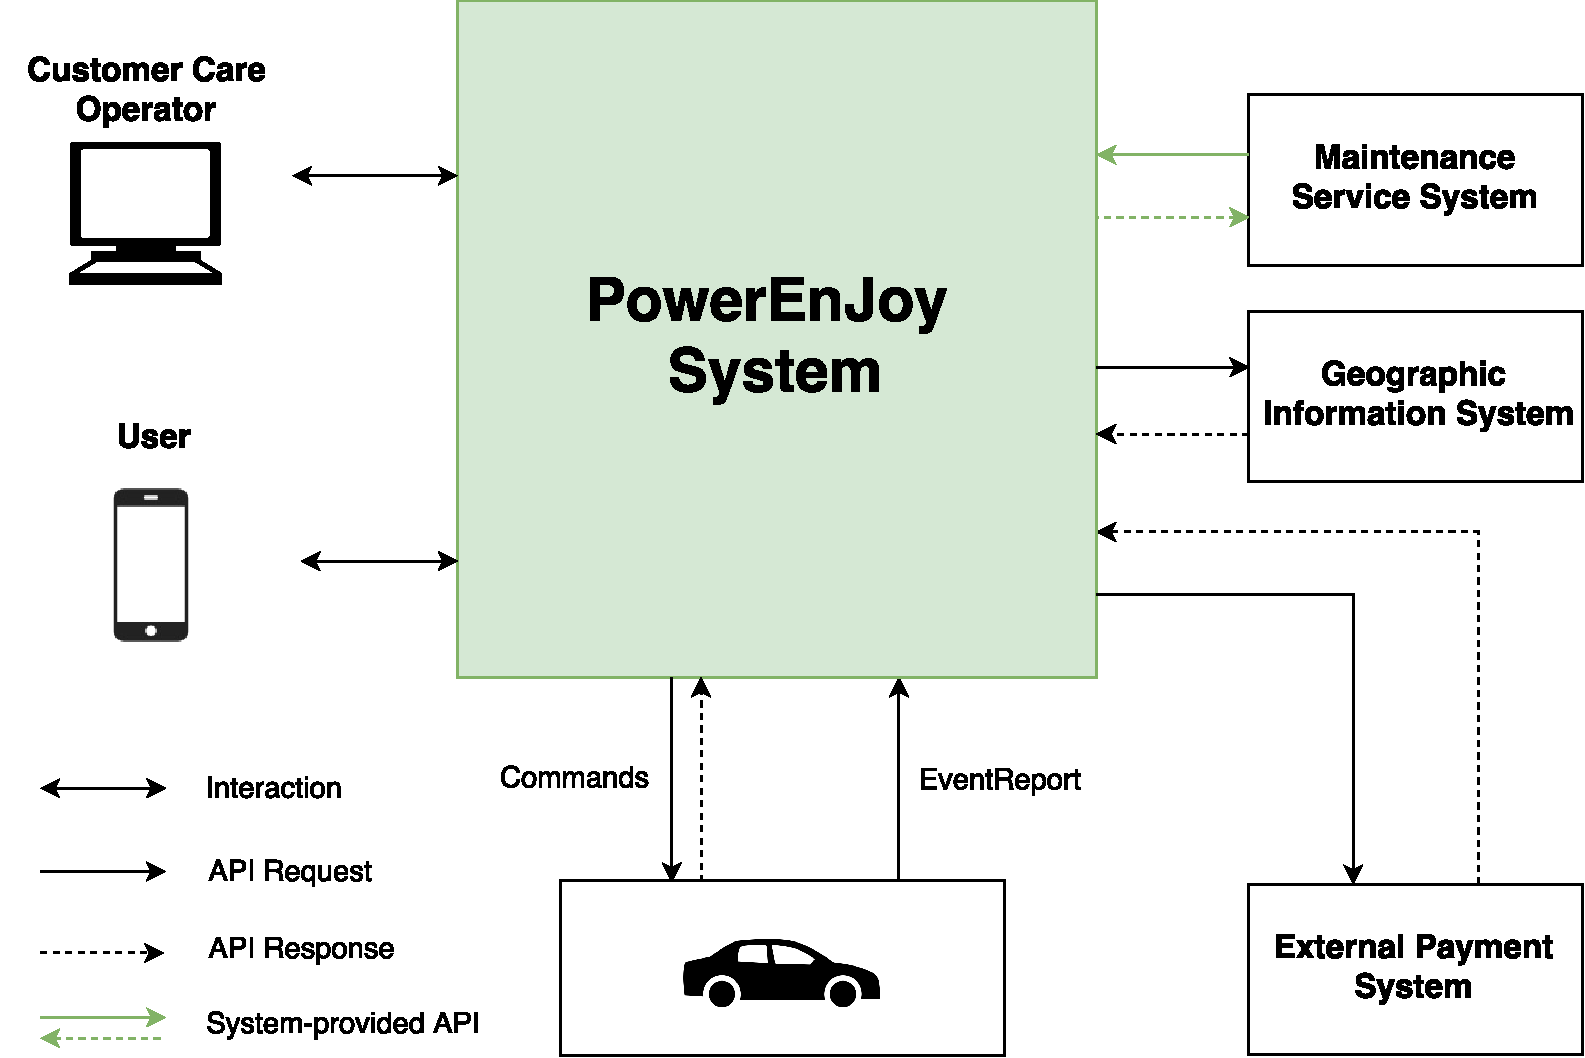
\includegraphics[width=\linewidth]{contextViewPoint}
			\caption{
				\label{fig:contextViewPoint} 
				Context viewpoint
			}
		\end{figure}
		
		We need to design a system which allows communications with many agents such as cars, users, external systems, etc.
		Moreover we recognize that in most of the interactions the system is providing a service to agents so, after taking in consideration different alternatives, we decided to use a client-server architectural approach.
		
		Cars offer to the system a set of primitives which allow it to interact with them: in this case it is clear that cars are providing the system services, so they can be identified as serves while the system acts as a client; on the other end the notification functionality offered by cars clearly yields to an event-based approach due to the asynchronous nature of such interactions, this led us to use a publish-subscribe paradigm for these specific interactions.
		\clearpage
		
	\subsubsection{Composition viewpoint}
	
		\begin{figure}[h]
			\centering
			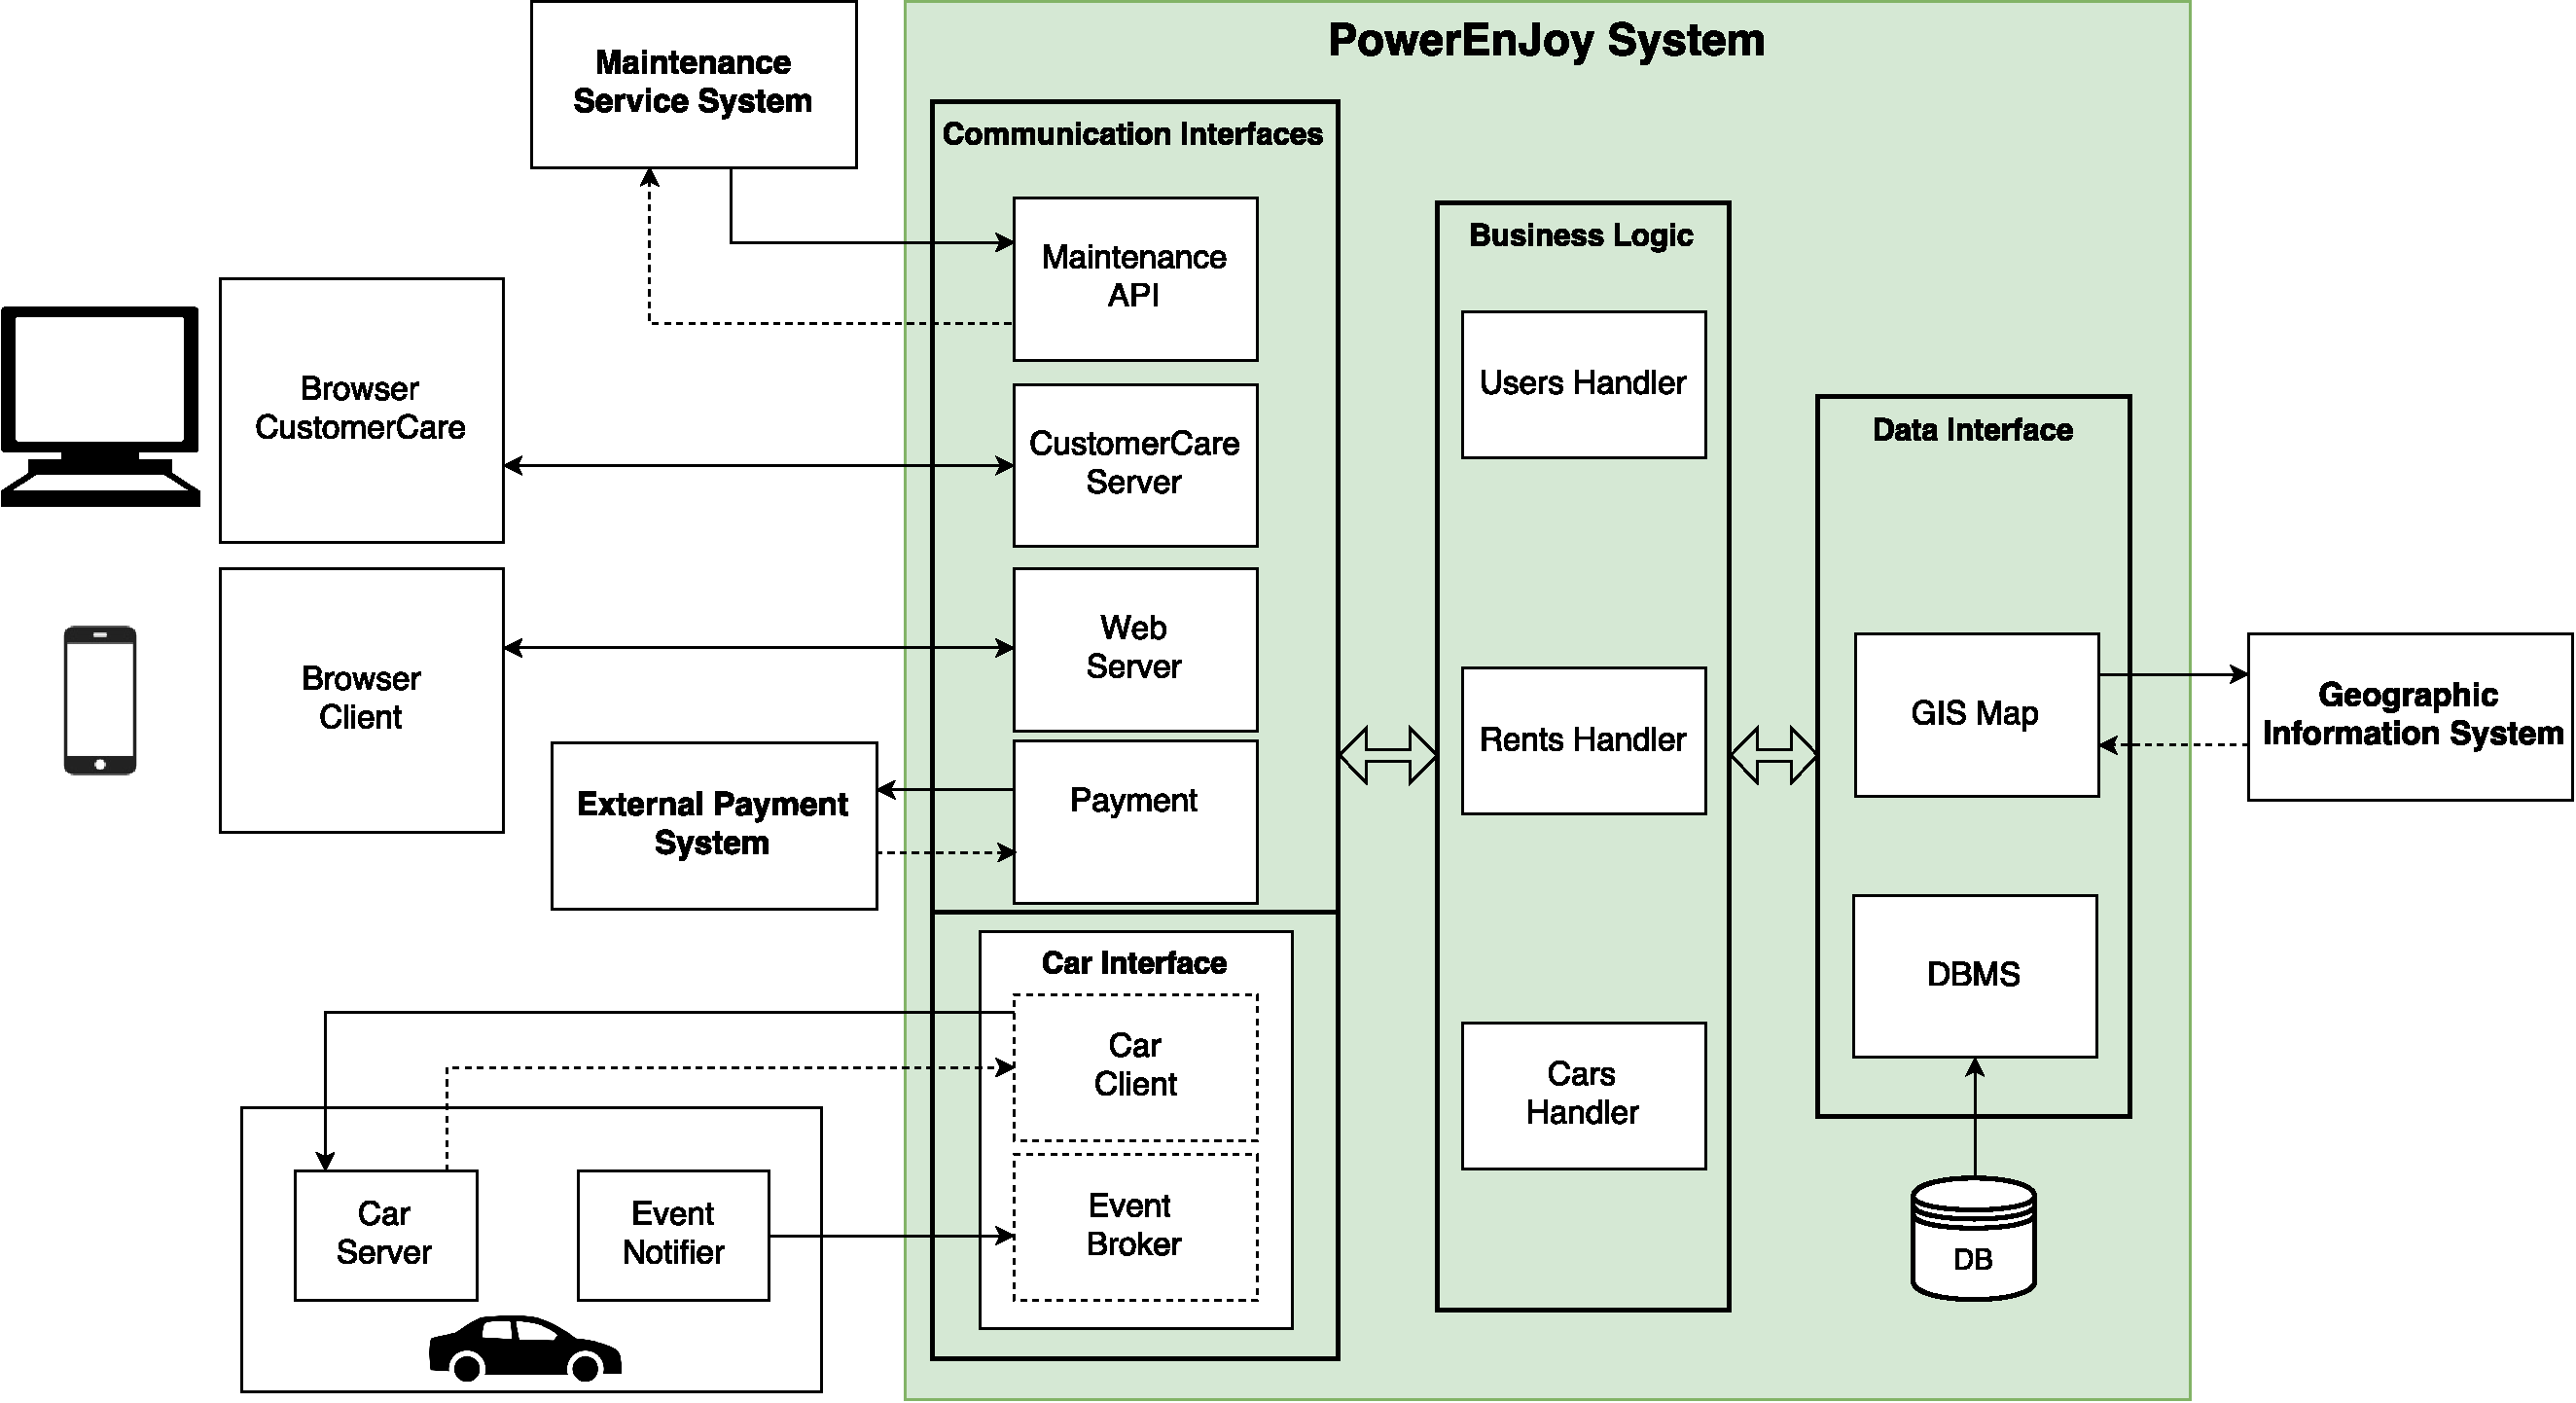
\includegraphics[width=\linewidth]{ComponentOverview}
			\caption{
				\label{fig:contextViewPoint} 
				Composition viewpoint
			}
		\end{figure}
		
		Going deeper in the analysis of our system composition, we are able to identify some of the modules that will be required in order to provide the functionalities specified in the Requirement Analysis and Specification Document. 
		\paragraph{Communication Interfaces}
			Since our system interacts with many external agents, it needs to have different \emph{Communication Interfaces} in order to communicate with them. 
		\begin{itemize}
			\item An API is needed to provide \emph{Maintenance Service System} the information it needs to work with us
			\item A software module is needed to provide the \emph{Customer Care} the functionalitities it needs
			\item A web server is needed in order to communicate with the users
			\item An internal payment software module will deal with the communication with the \emph{External Payment System} 
			\item A set of modules will manage the communications between the cars and the system;
		\end{itemize}
		\paragraph{Business Logic}
			The actual application logic of our system needs to manage the users information, the rents and the cars information; for each of these purposes several software modules are necessary; they will use communication interfaces to communicate with the agents and they will be able to retrieve data from the data interfaces.
		\paragraph{Data Interface}
			Our system needs a way to access and store the data it produces or retrieves from external resources, that is why \emph{Data Interface} modules are needed. These modules allows interaction between the \emph{Business Logic} modules and the System Databases; moreover they provide an interface to communicate with the GIS in order to allow the \emph{Business Logic} modules to access its functionalities.

\clearpage

\subsection{Component view}
\begin{figure}[h]
	\centering
	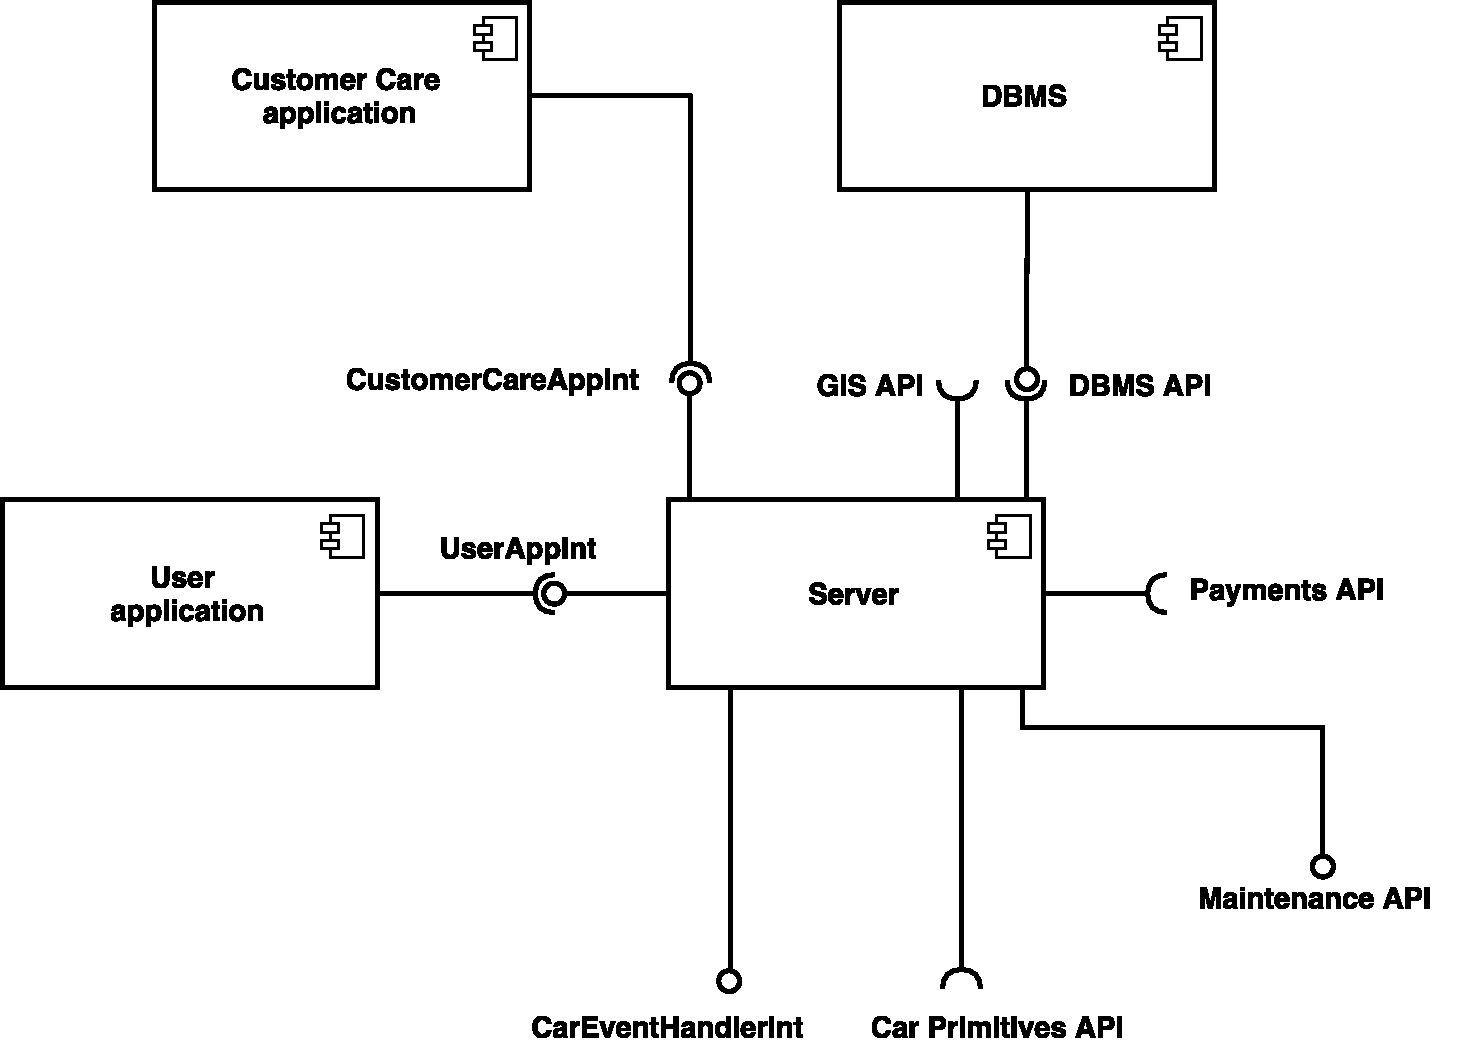
\includegraphics[width=\linewidth]{highLevelComponents}
	\caption{
		\label{fig:highLevelComponents} 
		High-level components
	}
\end{figure}
Considering all the previous graphs, we have identified in \autoref{fig:highLevelComponents} the following high level components, interfaces and mapping of the functionality defined in the RASD:
\begin{itemize}

	\item User application
	\begin{itemize}
		\item Register
		\item Login
		\item View the map with the position of
		\begin{itemize}
			\item himself
			\item safe areas
			\item available cars (with their battery level)
			\item charging stations
		\end{itemize}
		\item Reserve a car
		\item View customer care contacts
		\item Unlock the reserved car
		\item View and edit personal information
		\item View rents and payments history
	\end{itemize}
	
	\item Customer Care application
	\begin{itemize}
		\item View each user profile, including personal information, progress of the current rent, rent and payments history
		\item Mark and unmark users as banned
		\item Mark cars as Not Available
	\end{itemize}
	
	\item DBMS
	\begin{itemize}
		\item Store and retrieve data
	\end{itemize}	
	
	\item GIS API
	\begin{itemize}
		\item Get a map which will be populated with markers
	\end{itemize}
	
	\item Payments API
	\begin{itemize}
		\item Execute payment transactions
	\end{itemize}
	
	\item Maintenance API
	\begin{itemize}
		\item Expose the list of the cars tagged as Not Available with their GPS position and a brief description of the problem
		\item Tag Not Available cars as Available
	\end{itemize}
	
	\item Car Primitives API
	\begin{itemize}
		\item Call car embedded system's primitives
	\end{itemize}
	
	\item Car Event Handler Interface \todo{name must be consistent with graph}
	\begin{itemize}
		\item Triggered by an event notification from cars
	\end{itemize}
\end{itemize}
\clearpage

\subsubsection{Server Component}
To explain how the Server component manages interfaces, communication with external components and system functionalities we identify the main components inside the Server component and their interactions.
\\

\begin{figure}[h]
			\centering
			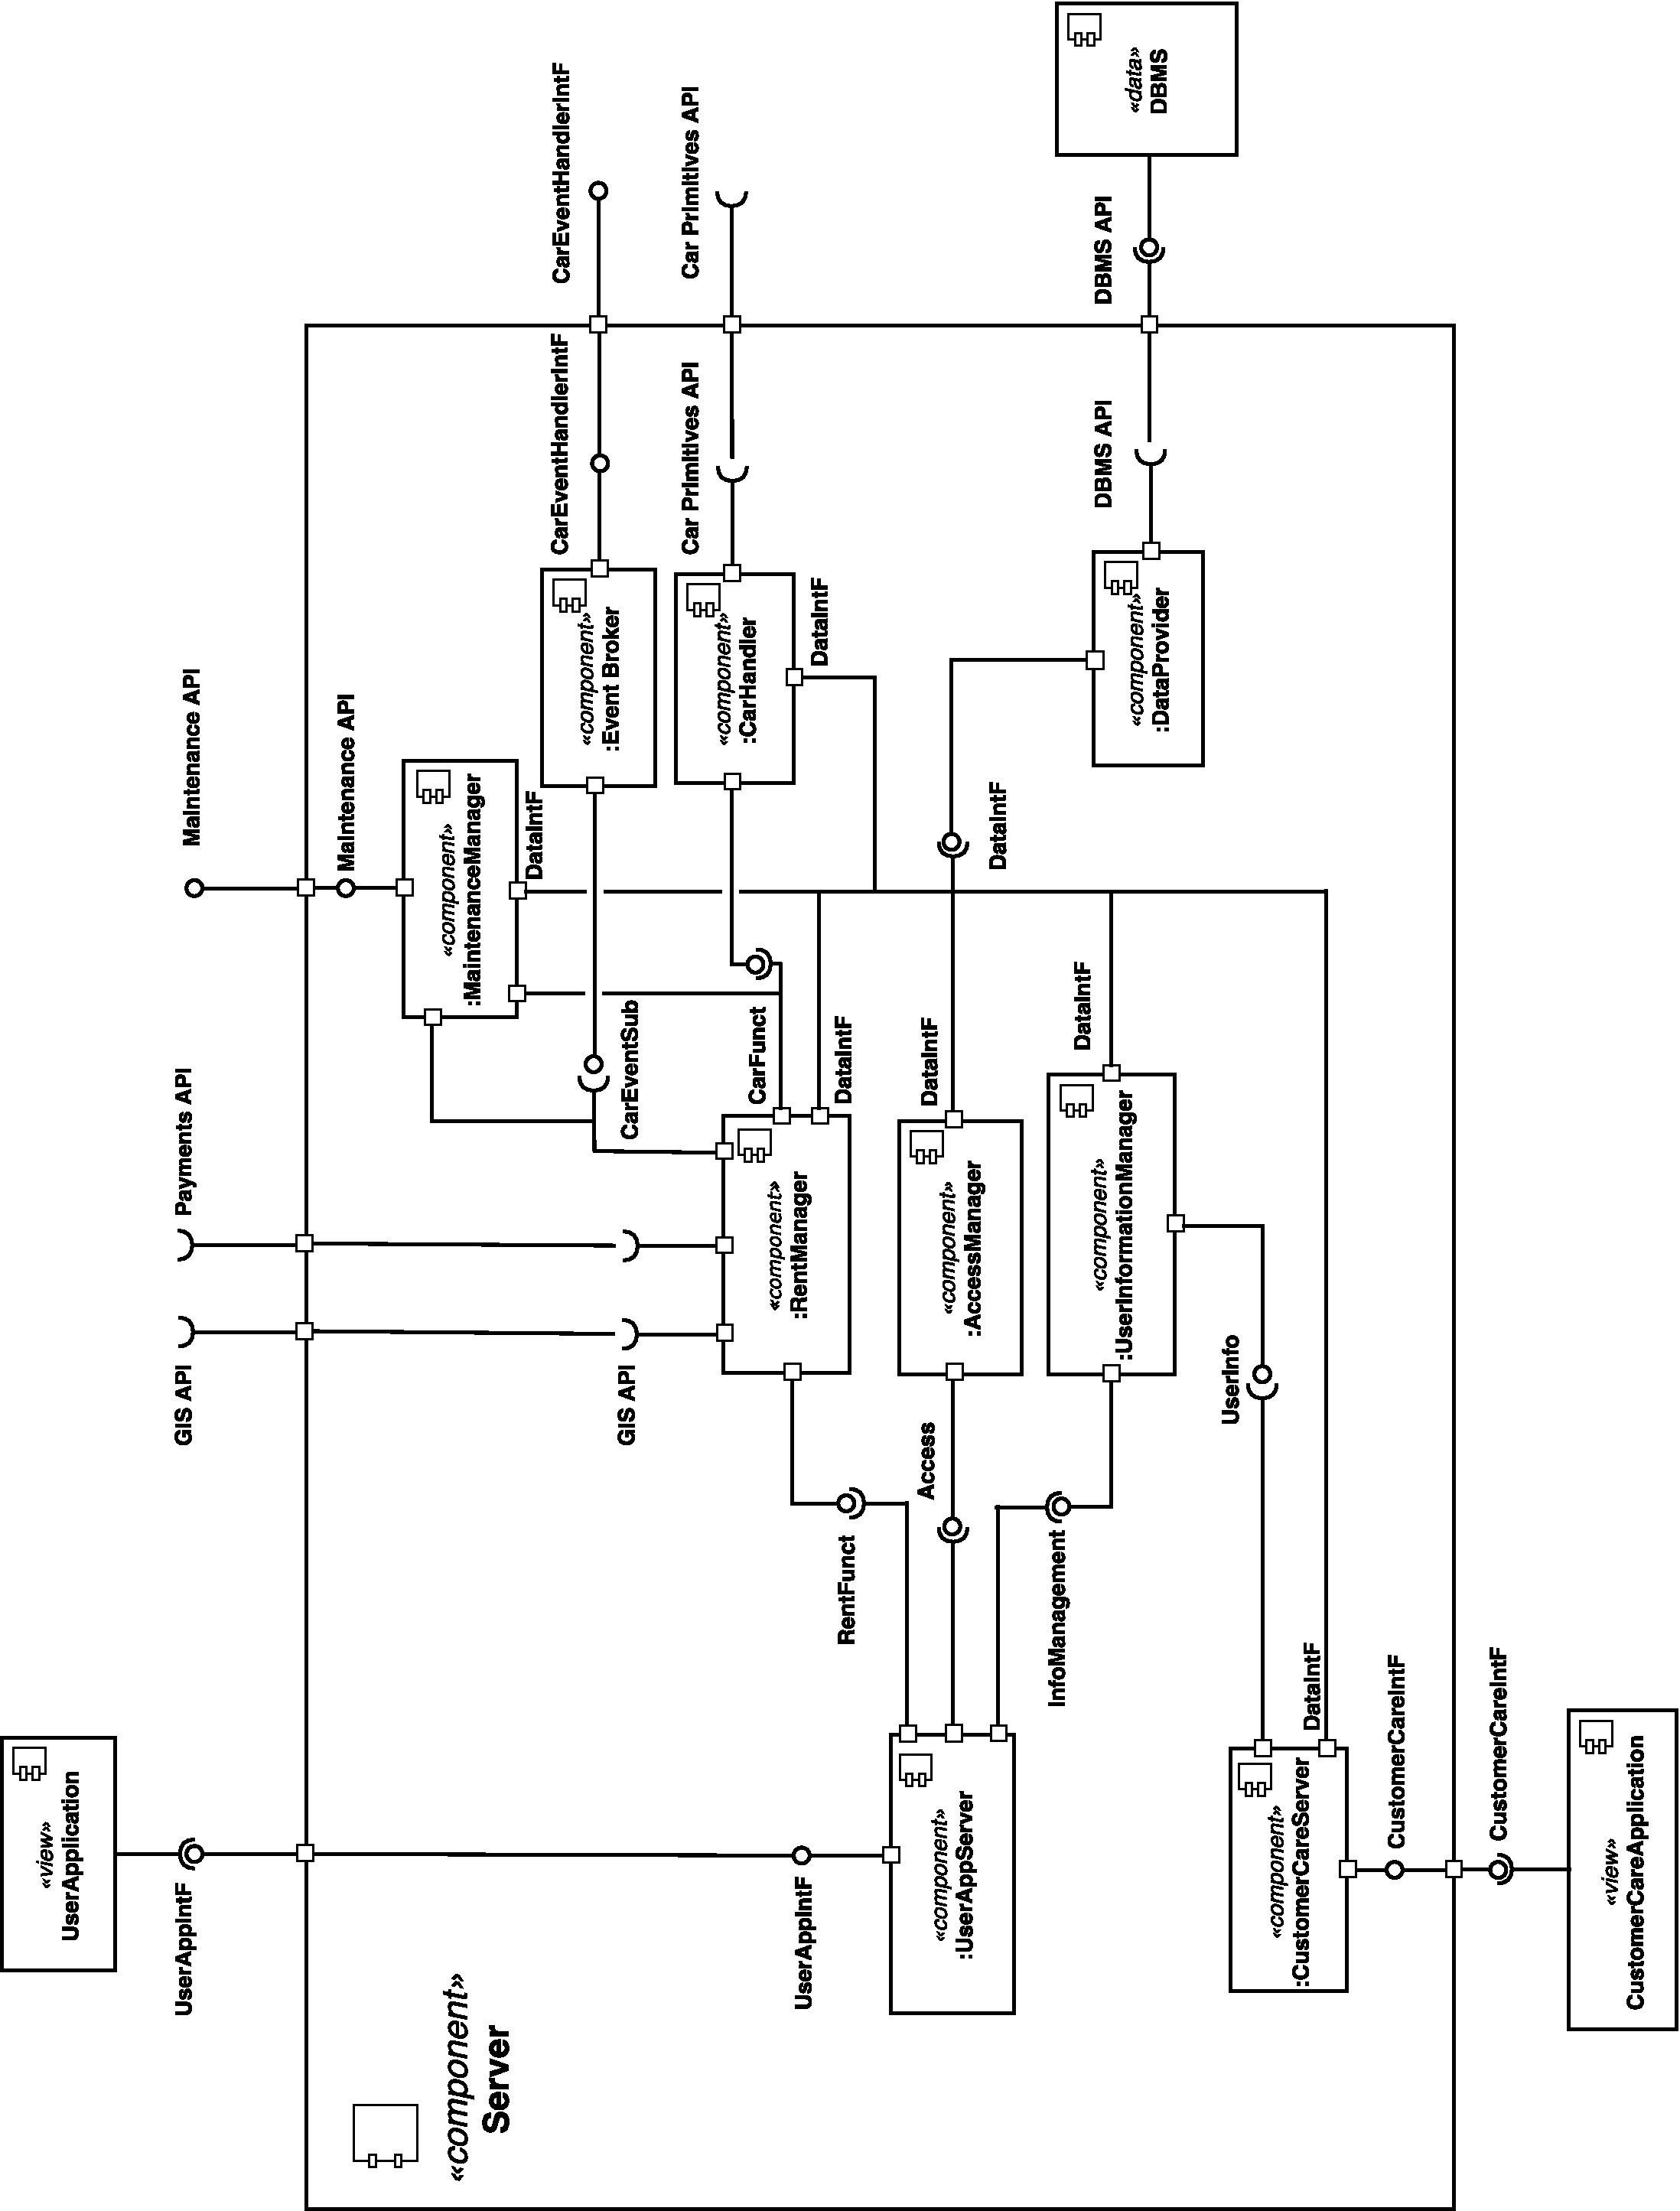
\includegraphics[width=0.9725\linewidth]{ServerComponent}
			\caption{
				\label{fig:ServerComponent} 
				Server component
			}
		\end{figure}
\clearpage

\subsection{Deployment view}
\subsection{Runtime view}
\subsection{Component interfaces}
\subsection{Architectural style and patterns}
\subsection{Other design decision}
